\author{Maciej Sobczynski}
\date{\today}

\title{\vspace{-2.0cm}Task 20\\Implement the Homeier method for finding a root of the polynomial $p(x)=c_0U_0(x)+c_1U_1(x)+...+c_nU_n(x)$, where $U_k(x)$ denotes the Chebyshev polynomial of the second order}
\documentclass[12pt]{article}
\usepackage{listings}  
\usepackage{amsfonts}
\usepackage{graphicx}
\providecommand{\e}[1]{\ensuremath{\times 10^{#1}}}
\begin{document}
\lstset{language=Matlab}
\maketitle

\section{Method description}
Homeier's method is a modified version of Newton's method for finding roots of polynomials so to understand it, we need to understand the Newton's method first.
\subsection{Newton's method}
The main idea of this method is to start with an initial guess for a root and then approximate the function by its tangent line. The next point is chosen at the intersection of the tangent and the $x$-axis. This point is the next (typically better) approximation of the function's root. This method can be iterated in the following fashion:\\
Let $f$ be a differentiable function with $x \in \mathbb{R}$ and $f(x)\in\mathbb{R}$. Suppose we already obtained current approximation $x_n$. Then the next approximation $x_{n+1}$ can be found. The tangent line to $y=f(x)$ at point $x=x_n$ is $$y=f'(x_n)(x-x_n)+f(x_n).$$ Next, the $x$-intercept of the tangent is used to find the approximation of the root $x_{n+1}$. We obtain it by solving the previous equation with $y=0$ and $x=x_{n+1}$ for $x_{n+1}$ which gives $$x_{n+1}=x_n-\frac{f(x_n)}{f'(x_n)}$$
\subsection{Hoimier's method}
This method is very similar to the previously explained Newton's method. The only key difference is that in this method $$x_{n+1}=x_n-\frac{1}{2}f(x_n)(\frac{1}{f'(x_n)}+\frac{1}{f'(y_n)})$$ where $$y_n=x_n-\frac{f(x_n)}{f'(x_n)}$$
\subsection{Chebyshev polynomials}
The Chebyshev polynomials are a sequence of polynomials related to the trigonometric multi-angle formulae. One usually distinguishes between Chebyshev polynomials of the first kind which are denoted $T_n$ and Chebyshev polynomials of the second kind which are denoted $U_n$.\\ \\
The Chebyshev polynomials of the second kind are defined by the recurrence relation $$U_0(x)=1$$ $$U_1(x)=2x$$ $$U_{n+1}(x)=2xU_n(x)-U_{n-1}(x)$$\\
The ordinary generating function for $U_n$ is $$\sum\limits_{n=0}^\infty U_n(x)t^n=\frac{1}{1-2tx+t^2}$$
and the exponential generating function is $$\sum\limits_{n=0}^\infty Y_n(x)\frac{t^n}{n!}=e^{tx}(\cosh(t\sqrt{x^2-1})+\frac{x}{\sqrt{x^2-1}}\sinh(t\sqrt{x^2-1})).$$
The first few Chebyshev polynomials of the second kind are
$$U_0(x)	=	1	$$
$$U_1(x)	=	2x	$$
$$U_2(x)	=	4x^2-1	$$
$$U_3(x)	=	8x^3-4x	$$
$$U_4(x)	=	16x^4-12x^2+1	$$
$$U_5(x)	=	32x^5-32x^3+6x	$$
$$U_6(x)	=	64x^6-80x^4+24x^2-1$$

\section{Program description}
\subsection{Homeier.m}
A function to implement the Homeier's method. It takes four arguments: f - an input function, x0 - initial approximation/guess, tol - tolerance and max - maximal number of iterations. The function returns the approximation of the root and number of iterations.
\subsection{Cheby.m}
A function to calculate the value of the polynomial$p(x)=c_0U_0(x)+c_1U_1(x)+...+c_nU_n(x)$ and it's derivative. As an input argument, the function takes a vector of coefficients that represents $c_0, c_1, ..., c_n$ and value $x$ at which the polynomial is evaluated. The function returns two values - p -value of the polynomial and p2 - value of it's derivative)
\subsection{Scripts}
The scripts contain the numerical examples presented in the next section
\section{Numerical examples}
In the examples the function will be graphed and the result of the Homeier method $x_0$ and number of iterations $k$ will be presented as well as $diff$ - the value of the polynomial at $x_0$
\subsection{Example 1}
\begin{figure}[!htb]
\centering
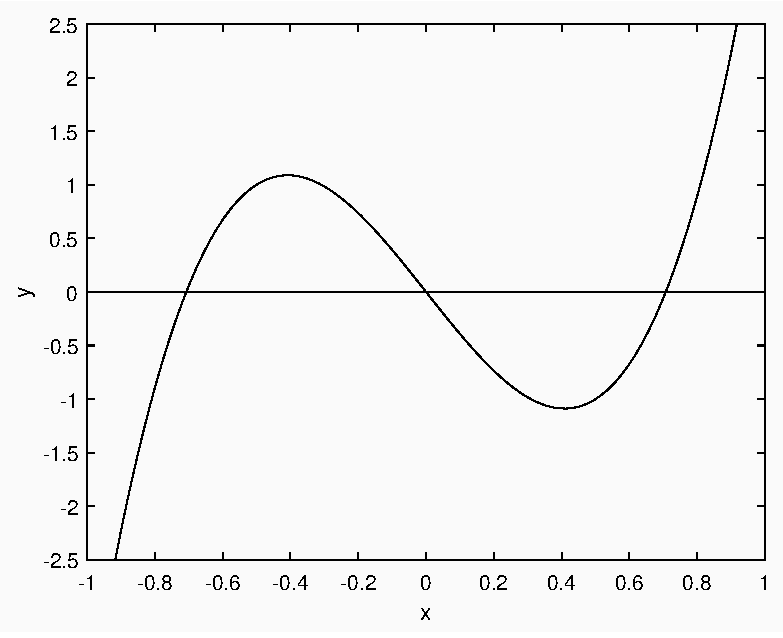
\includegraphics[width=110mm]{ex1}
\caption{Example 1 graph}
\end{figure}
x0 = 0.3090,
k = 5,
diff = -2.2204e-16
\lstinputlisting{Example1.m}
\subsection{Example 2}
\begin{figure}[!htb]
\centering
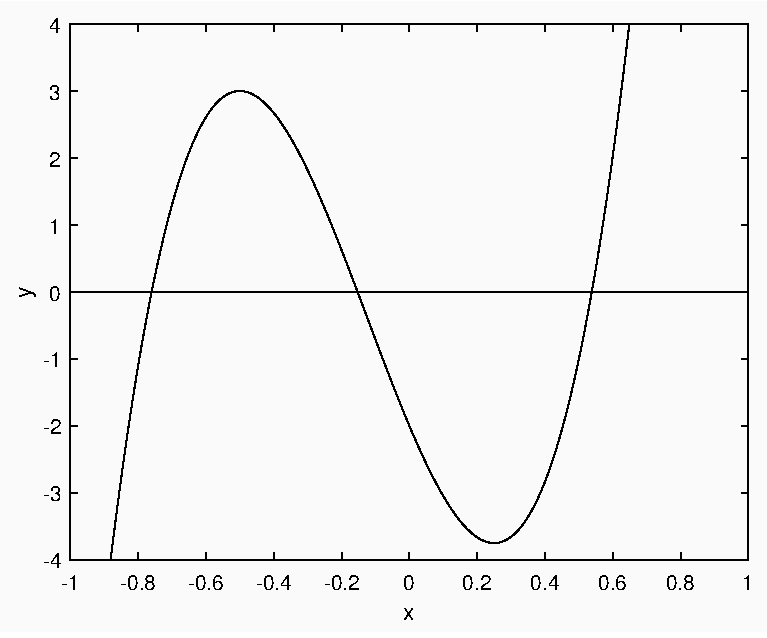
\includegraphics[width=110mm]{ex2}
\caption{Example 2 graph}
\end{figure}
x0 = -0.1528,
k = 3,
diff = 4.3350e-06
\lstinputlisting{Example2.m}
\subsection{Example 3}
\begin{figure}[!htb]
\centering
\includegraphics[width=110mm]{ex3}
\caption{Example 3 graph}
\end{figure}
x0 = 0.2570,
k = 3,
diff = 0
\lstinputlisting{Example3.m}
\subsection{Example 4}
\begin{figure}[!htb]
\centering
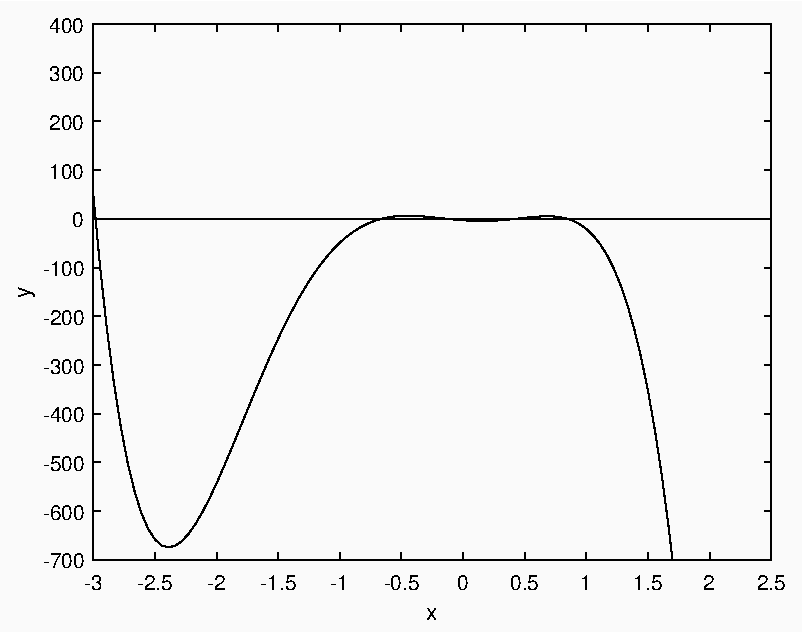
\includegraphics[width=110mm]{ex4}
\caption{Example 4 graph}
\end{figure}
x0 = 0.8464,
k = 9,
diff = 2.2204e-15
\lstinputlisting{Example4.m}
\section{Analysis of results}
Overall the Homeier method provides an extremely fast way of of finding the roots of a polynomial. The method is quite precise and fast - the number of iterations is usually very low.

\section{Code}
\subsection{Homeier.m}
\lstinputlisting{Homeier.m}
\subsection{Cheby.m}
\lstinputlisting{Cheby.m}
\bibliography{main}

\end{document}
  